\documentclass{homework}

\usepackage{wrapfig}
\usepackage{float}
\usepackage{indentfirst}
\usepackage{apacite}

\title{Actividad 5}
\date{2020-01-17}
\gdate{TAV 2020}
\author{Nicholas Mc-Donnell}
\course{Programa de Habilidades Comunicativas Escritas\\ para Ciencias Naturales y Matemáticas - LET172E}

\setlength{\parindent}{2em}
\setlength{\parskip}{1em}
\renewcommand{\baselinestretch}{1.5}
\newcommand{\tm}{\textsuperscript{TM}}

\begin{document}
\renewcommand{\BOthers}[1]{et al.\hbox{}}
\maketitle

El ``Machine Learning'' se ha vuelto una vital herramienta para múltiples tipos de problemas, desde  clasificación de imágenes \cite{DBLP:journals/corr/abs-1905-03288} hasta ayudar a traducir documentos. En este último, las Redes Neuronales (RNs)\footnote{La tecnología detrás del ``Machine Learning''} han sido un cambio impresionante al área, cada persona que ha usado Google Translate\tm ha notado la impresionante mejora en los últimos años, en los cuales el servicio transicionó de usar ``Statistical Machine Learning'' a RNs \fullcite{GoogleTranslate}.

El gran cambio que se ha visto viene de la reciente investigación en distintas arquitecturas de RNs, por ejemplo \fullciteA{rashid2019bilingualgan} propusieron un modelo el cual utiliza avances en otro problema\footnote{El problema de procesamiento de lenguaje natural (NLP).} para además avanzar en la calidad de traducción, otros como \fullciteA{vaswani2017attention} proponen un modelo simple usando el ``Transformador'' como base. Esto claramente muestra una variedad importante en las arquitecturas de RNs que intentan solucionar el problema de traducción.

Por lo cual, este trabajo tiene el objetivo de comparar distintas arquitecturas de Redes Neuronales para el problema de mapeo multilingüe\footnote{i.e, uno de los problemas asociados al problema de traducción}. Para lograr esto, se realizó una revisión de literatura de varios artículos sobre el tema, de los cuales tres tienen como enfoque presentar una nueva arquitectura de RNs y el resto da mejoras y apoyo a los primeros. Para un facilitar la comparación se introducirán las distintas arquitecturas separadamente, primero se verá la arquitectura de \shortciteA{vaswani2017attention}, después la de \shortciteA{rashid2019bilingualgan} y por último la de \shortciteA{artetxe2018robust}, después de introducirlas se hará una comparación de los resultados de cada arquitectura.
% TODO add number of papers cited

\subsection*{El Transformador, arquitectura de \shortciteA{vaswani2017attention}}

La arquitectura presentada por \shortciteA{vaswani2017attention} es una que solamente usa un mecanismo de atención entre el decodificador y el codificador, a este la llaman el Transformador. La idea solo usar el mecanismo de atención proviene de artículos anteriores donde se usaban arquitecturas de RNs convolucionales que incluían un decodificador y un codificador, pero además agregaban un mecanismo de atención entre el decodificador y el codificador, logrando así mejores resultados que las RNs convolucionales que no usan este mecanismo.

Para profundizar, el Transformador tiene dos partes, el decodificador y el codificador. El codificador mapea una secuencia de representaciones con símbolos \(\paren{x_1,\dots,x_n}\) a una secuencia de representación continua \(z=\paren{z_1,\dots,z_n}\)\footnote{i.e., es un punto en \(\set{R}^n\)}. El decodificador a su vez, toma \(z\) y genera una secuencia de símbolos \(\paren{y_1,\dots,y_m}\) un símbolo a la vez. Agregando a lo anterior, el modelo es auto-regresivo en cada paso, en otras palabras el modelo usa de input el símbolo generado anteriormente para generar el siguiente símbolo. Como se ve en la \nameref{fig1:attention}, lo anterior se traduce en en módulos de ``Atención Multi-Cabezal'', de ``Atención Multi-Cabezal Enmáscarada'', de ``Retroalimentación'' y por último de ``Softmax''. De estos, el de mayor interés es el de Atención Multi-Cabezal, este puede verse como una función que mapea una consulta y un conjunto de pares llave-valor a una salida, donde la consulta, las llaves y los valores son vectores. En este módulo es donde aparecen grandes mejoras, ya que este modulo es altamente paralelizable, lo que se traduce a una reducción importante de la cantidad de horas que se necesitan para entrenar el modelo completo.

\subsection*{GAN Bilingüe, arquitectura de \shortciteA{rashid2019bilingualgan}}

\section*{Figuras}
\begin{figure}[H]
    \caption{Fig. 1 del artículo de \protect\cite{vaswani2017attention}}
    \centering
    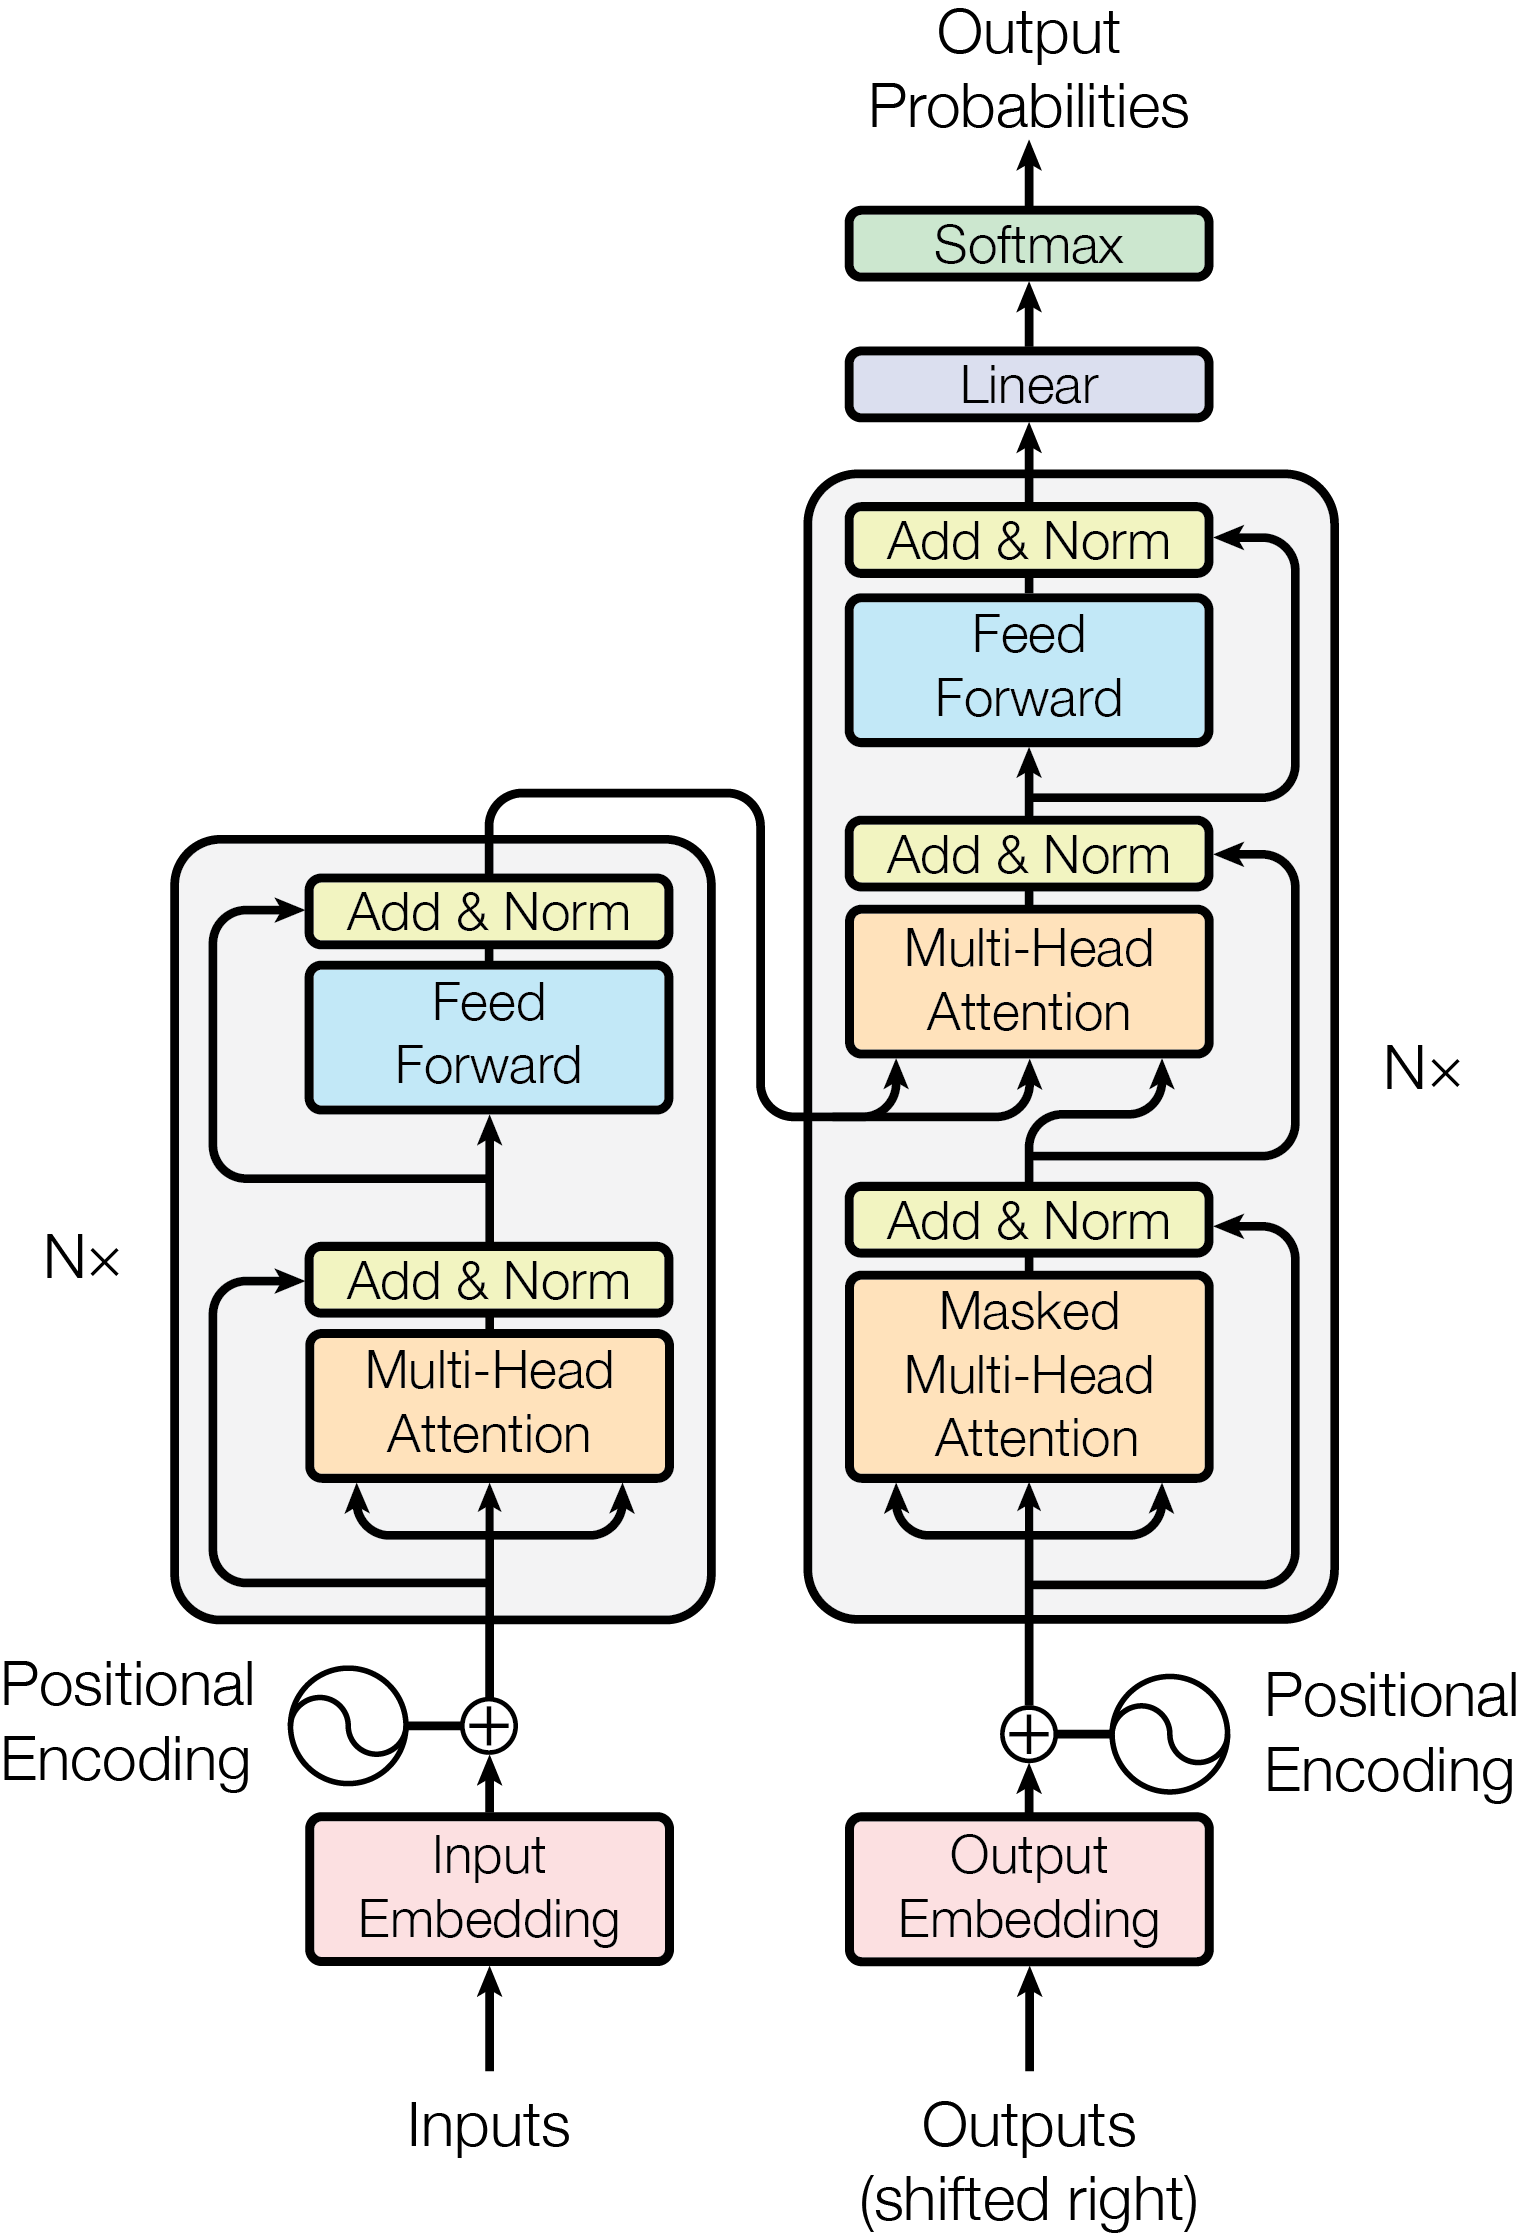
\includegraphics[width=0.5\textwidth]{Fig1.png}
    \label{fig1:attention}
\end{figure}

\bibliographystyle{apacite}
\bibliography{ref}

\end{document}